% Options for packages loaded elsewhere
\PassOptionsToPackage{unicode}{hyperref}
\PassOptionsToPackage{hyphens}{url}
%
\documentclass[
]{article}
\usepackage{amsmath,amssymb}
\usepackage{lmodern}
\usepackage{ifxetex,ifluatex}
\ifnum 0\ifxetex 1\fi\ifluatex 1\fi=0 % if pdftex
  \usepackage[T1]{fontenc}
  \usepackage[utf8]{inputenc}
  \usepackage{textcomp} % provide euro and other symbols
\else % if luatex or xetex
  \usepackage{unicode-math}
  \defaultfontfeatures{Scale=MatchLowercase}
  \defaultfontfeatures[\rmfamily]{Ligatures=TeX,Scale=1}
\fi
% Use upquote if available, for straight quotes in verbatim environments
\IfFileExists{upquote.sty}{\usepackage{upquote}}{}
\IfFileExists{microtype.sty}{% use microtype if available
  \usepackage[]{microtype}
  \UseMicrotypeSet[protrusion]{basicmath} % disable protrusion for tt fonts
}{}
\makeatletter
\@ifundefined{KOMAClassName}{% if non-KOMA class
  \IfFileExists{parskip.sty}{%
    \usepackage{parskip}
  }{% else
    \setlength{\parindent}{0pt}
    \setlength{\parskip}{6pt plus 2pt minus 1pt}}
}{% if KOMA class
  \KOMAoptions{parskip=half}}
\makeatother
\usepackage{xcolor}
\IfFileExists{xurl.sty}{\usepackage{xurl}}{} % add URL line breaks if available
\IfFileExists{bookmark.sty}{\usepackage{bookmark}}{\usepackage{hyperref}}
\hypersetup{
  pdftitle={Assignments},
  hidelinks,
  pdfcreator={LaTeX via pandoc}}
\urlstyle{same} % disable monospaced font for URLs
\usepackage[margin=1in]{geometry}
\usepackage{color}
\usepackage{fancyvrb}
\newcommand{\VerbBar}{|}
\newcommand{\VERB}{\Verb[commandchars=\\\{\}]}
\DefineVerbatimEnvironment{Highlighting}{Verbatim}{commandchars=\\\{\}}
% Add ',fontsize=\small' for more characters per line
\usepackage{framed}
\definecolor{shadecolor}{RGB}{248,248,248}
\newenvironment{Shaded}{\begin{snugshade}}{\end{snugshade}}
\newcommand{\AlertTok}[1]{\textcolor[rgb]{0.94,0.16,0.16}{#1}}
\newcommand{\AnnotationTok}[1]{\textcolor[rgb]{0.56,0.35,0.01}{\textbf{\textit{#1}}}}
\newcommand{\AttributeTok}[1]{\textcolor[rgb]{0.77,0.63,0.00}{#1}}
\newcommand{\BaseNTok}[1]{\textcolor[rgb]{0.00,0.00,0.81}{#1}}
\newcommand{\BuiltInTok}[1]{#1}
\newcommand{\CharTok}[1]{\textcolor[rgb]{0.31,0.60,0.02}{#1}}
\newcommand{\CommentTok}[1]{\textcolor[rgb]{0.56,0.35,0.01}{\textit{#1}}}
\newcommand{\CommentVarTok}[1]{\textcolor[rgb]{0.56,0.35,0.01}{\textbf{\textit{#1}}}}
\newcommand{\ConstantTok}[1]{\textcolor[rgb]{0.00,0.00,0.00}{#1}}
\newcommand{\ControlFlowTok}[1]{\textcolor[rgb]{0.13,0.29,0.53}{\textbf{#1}}}
\newcommand{\DataTypeTok}[1]{\textcolor[rgb]{0.13,0.29,0.53}{#1}}
\newcommand{\DecValTok}[1]{\textcolor[rgb]{0.00,0.00,0.81}{#1}}
\newcommand{\DocumentationTok}[1]{\textcolor[rgb]{0.56,0.35,0.01}{\textbf{\textit{#1}}}}
\newcommand{\ErrorTok}[1]{\textcolor[rgb]{0.64,0.00,0.00}{\textbf{#1}}}
\newcommand{\ExtensionTok}[1]{#1}
\newcommand{\FloatTok}[1]{\textcolor[rgb]{0.00,0.00,0.81}{#1}}
\newcommand{\FunctionTok}[1]{\textcolor[rgb]{0.00,0.00,0.00}{#1}}
\newcommand{\ImportTok}[1]{#1}
\newcommand{\InformationTok}[1]{\textcolor[rgb]{0.56,0.35,0.01}{\textbf{\textit{#1}}}}
\newcommand{\KeywordTok}[1]{\textcolor[rgb]{0.13,0.29,0.53}{\textbf{#1}}}
\newcommand{\NormalTok}[1]{#1}
\newcommand{\OperatorTok}[1]{\textcolor[rgb]{0.81,0.36,0.00}{\textbf{#1}}}
\newcommand{\OtherTok}[1]{\textcolor[rgb]{0.56,0.35,0.01}{#1}}
\newcommand{\PreprocessorTok}[1]{\textcolor[rgb]{0.56,0.35,0.01}{\textit{#1}}}
\newcommand{\RegionMarkerTok}[1]{#1}
\newcommand{\SpecialCharTok}[1]{\textcolor[rgb]{0.00,0.00,0.00}{#1}}
\newcommand{\SpecialStringTok}[1]{\textcolor[rgb]{0.31,0.60,0.02}{#1}}
\newcommand{\StringTok}[1]{\textcolor[rgb]{0.31,0.60,0.02}{#1}}
\newcommand{\VariableTok}[1]{\textcolor[rgb]{0.00,0.00,0.00}{#1}}
\newcommand{\VerbatimStringTok}[1]{\textcolor[rgb]{0.31,0.60,0.02}{#1}}
\newcommand{\WarningTok}[1]{\textcolor[rgb]{0.56,0.35,0.01}{\textbf{\textit{#1}}}}
\usepackage{graphicx}
\makeatletter
\def\maxwidth{\ifdim\Gin@nat@width>\linewidth\linewidth\else\Gin@nat@width\fi}
\def\maxheight{\ifdim\Gin@nat@height>\textheight\textheight\else\Gin@nat@height\fi}
\makeatother
% Scale images if necessary, so that they will not overflow the page
% margins by default, and it is still possible to overwrite the defaults
% using explicit options in \includegraphics[width, height, ...]{}
\setkeys{Gin}{width=\maxwidth,height=\maxheight,keepaspectratio}
% Set default figure placement to htbp
\makeatletter
\def\fps@figure{htbp}
\makeatother
\setlength{\emergencystretch}{3em} % prevent overfull lines
\providecommand{\tightlist}{%
  \setlength{\itemsep}{0pt}\setlength{\parskip}{0pt}}
\setcounter{secnumdepth}{-\maxdimen} % remove section numbering
\ifluatex
  \usepackage{selnolig}  % disable illegal ligatures
\fi

\title{Assignments}
\author{}
\date{\vspace{-2.5em}}

\begin{document}
\maketitle

This page will contain all the assignments you submit for the class.

\hypertarget{instructions-for-all-assignments}{%
\subsubsection{Instructions for all
assignments}\label{instructions-for-all-assignments}}

I want you to submit your assignment as a PDF, so I can keep a record of
what the code looked like that day. I also want you to include your
answers on your personal GitHub website. This will be good practice for
editing your website and it will help you produce something you can keep
after the class is over.

\begin{enumerate}
\def\labelenumi{\arabic{enumi}.}
\item
  Download the Assignment1.Rmd file from Canvas. You can use this as a
  template for writing your answers. It's the same as what you can see
  on my website in the Assignments tab. Once we're done with this I'll
  edit the text on the website to include the solutions.
\item
  On RStudio, open a new R script in RStudio (File \textgreater{} New
  File \textgreater{} R Script). This is where you can test out your R
  code. You'll write your R commands and draw plots here.
\item
  Once you have finalized your code, copy and paste your results into
  this template (Assignment 1.Rmd). For example, if you produced a plot
  as the solution to one of the problems, you can copy and paste the R
  code in R markdown by using the
  \texttt{\textasciigrave{}\textasciigrave{}\{r\}\ \textasciigrave{}\textasciigrave{}\textasciigrave{}}
  command. Answer the questions in full sentences and Save.
\item
  Produce a PDF file with your answers. To do this, knit to PDF (use
  Knit button at the top of RStudio), locate the PDF file in your docs
  folder (it's in the same folder as the Rproj), and submit that on on
  Canvas in Assignment 1.
\item
  Build Website, go to GitHub desktop, commit and push. Now your
  solutions should be on your website as well.
\end{enumerate}

\hypertarget{assignment-1}{%
\section{Assignment 1}\label{assignment-1}}

\textbf{Collaborators: }

\hypertarget{problem-1}{%
\subsubsection{Problem 1}\label{problem-1}}

Install the datasets package on the console below using
\texttt{install.packages("datasets")}. Now load the library.

\begin{Shaded}
\begin{Highlighting}[]
\CommentTok{\#install.packages("datasets")}
\FunctionTok{library}\NormalTok{(datasets)}

\NormalTok{USArrests}
\end{Highlighting}
\end{Shaded}

\begin{verbatim}
##                Murder Assault UrbanPop Rape
## Alabama          13.2     236       58 21.2
## Alaska           10.0     263       48 44.5
## Arizona           8.1     294       80 31.0
## Arkansas          8.8     190       50 19.5
## California        9.0     276       91 40.6
## Colorado          7.9     204       78 38.7
## Connecticut       3.3     110       77 11.1
## Delaware          5.9     238       72 15.8
## Florida          15.4     335       80 31.9
## Georgia          17.4     211       60 25.8
## Hawaii            5.3      46       83 20.2
## Idaho             2.6     120       54 14.2
## Illinois         10.4     249       83 24.0
## Indiana           7.2     113       65 21.0
## Iowa              2.2      56       57 11.3
## Kansas            6.0     115       66 18.0
## Kentucky          9.7     109       52 16.3
## Louisiana        15.4     249       66 22.2
## Maine             2.1      83       51  7.8
## Maryland         11.3     300       67 27.8
## Massachusetts     4.4     149       85 16.3
## Michigan         12.1     255       74 35.1
## Minnesota         2.7      72       66 14.9
## Mississippi      16.1     259       44 17.1
## Missouri          9.0     178       70 28.2
## Montana           6.0     109       53 16.4
## Nebraska          4.3     102       62 16.5
## Nevada           12.2     252       81 46.0
## New Hampshire     2.1      57       56  9.5
## New Jersey        7.4     159       89 18.8
## New Mexico       11.4     285       70 32.1
## New York         11.1     254       86 26.1
## North Carolina   13.0     337       45 16.1
## North Dakota      0.8      45       44  7.3
## Ohio              7.3     120       75 21.4
## Oklahoma          6.6     151       68 20.0
## Oregon            4.9     159       67 29.3
## Pennsylvania      6.3     106       72 14.9
## Rhode Island      3.4     174       87  8.3
## South Carolina   14.4     279       48 22.5
## South Dakota      3.8      86       45 12.8
## Tennessee        13.2     188       59 26.9
## Texas            12.7     201       80 25.5
## Utah              3.2     120       80 22.9
## Vermont           2.2      48       32 11.2
## Virginia          8.5     156       63 20.7
## Washington        4.0     145       73 26.2
## West Virginia     5.7      81       39  9.3
## Wisconsin         2.6      53       66 10.8
## Wyoming           6.8     161       60 15.6
\end{verbatim}

Load the USArrests dataset and rename it \texttt{dat}. Note that this
dataset comes with R, in the package datasets, so there's no need to
load data from your computer. Why is it useful to rename the dataset?

It is useful to renamed USArrests to dat.us because it is easier to
write and it is good practice to rewrite data for yourself so you can
create your own data which can be replicated by another person if they
use the original data.

\begin{Shaded}
\begin{Highlighting}[]
\NormalTok{dat.us }\OtherTok{\textless{}{-}}\NormalTok{ USArrests}

\FunctionTok{head}\NormalTok{(dat.us)}
\end{Highlighting}
\end{Shaded}

\begin{verbatim}
##            Murder Assault UrbanPop Rape
## Alabama      13.2     236       58 21.2
## Alaska       10.0     263       48 44.5
## Arizona       8.1     294       80 31.0
## Arkansas      8.8     190       50 19.5
## California    9.0     276       91 40.6
## Colorado      7.9     204       78 38.7
\end{verbatim}

\hypertarget{problem-2}{%
\subsubsection{Problem 2}\label{problem-2}}

Use this command to make the state names into a new variable called
State.

\begin{Shaded}
\begin{Highlighting}[]
\NormalTok{dat}\SpecialCharTok{$}\NormalTok{state }\OtherTok{\textless{}{-}} \FunctionTok{tolower}\NormalTok{(}\FunctionTok{rownames}\NormalTok{(USArrests))}
\end{Highlighting}
\end{Shaded}

This dataset has the state names as row names, so we just want to make
them into a new variable. We also make them all lower case, because that
will help us draw a map later - the map function requires the states to
be lower case.

List the variables contained in the dataset \texttt{USArrests}.

\begin{Shaded}
\begin{Highlighting}[]
\FunctionTok{names}\NormalTok{(dat.us)}
\end{Highlighting}
\end{Shaded}

\begin{verbatim}
## [1] "Murder"   "Assault"  "UrbanPop" "Rape"
\end{verbatim}

Answer: The four variables are Murder, Assault, UrbanPop, Rape.

\hypertarget{problem-3}{%
\subsubsection{Problem 3}\label{problem-3}}

What type of variable (from the DVB chapter) is \texttt{Murder}?

Answer: Murder is a quantitative variable.

What R Type of variable is it?

Answer: Murder is numeric.

\hypertarget{problem-4}{%
\subsubsection{Problem 4}\label{problem-4}}

What information is contained in this dataset, in general? What do the
numbers mean?

Answer: The dataset contains the data of murder, assault, rape and
urbanpop from all 50 US states. The numbers represent the frequency of
arrests for one of the four variables in a state during the time frame
that the data was collected.

\hypertarget{problem-5}{%
\subsubsection{Problem 5}\label{problem-5}}

Draw a histogram of \texttt{Murder} with proper labels and title.

\begin{Shaded}
\begin{Highlighting}[]
\FunctionTok{hist}\NormalTok{(dat.us}\SpecialCharTok{$}\NormalTok{Murder, }\AttributeTok{xlab=} \StringTok{"Murders"}\NormalTok{, }\AttributeTok{ylab=}\StringTok{"Frequency"}\NormalTok{, }\AttributeTok{main=} \StringTok{"Murder in the US"}\NormalTok{, }\AttributeTok{xlim=}\NormalTok{(}\FunctionTok{c}\NormalTok{(}\DecValTok{0}\NormalTok{, }\DecValTok{20}\NormalTok{)), }\AttributeTok{ylim=}\NormalTok{(}\FunctionTok{c}\NormalTok{(}\DecValTok{0}\NormalTok{, }\DecValTok{13}\NormalTok{)), }\AttributeTok{col=}\StringTok{"red"}\NormalTok{, }\AttributeTok{breaks=} \DecValTok{10}\NormalTok{)}
\end{Highlighting}
\end{Shaded}

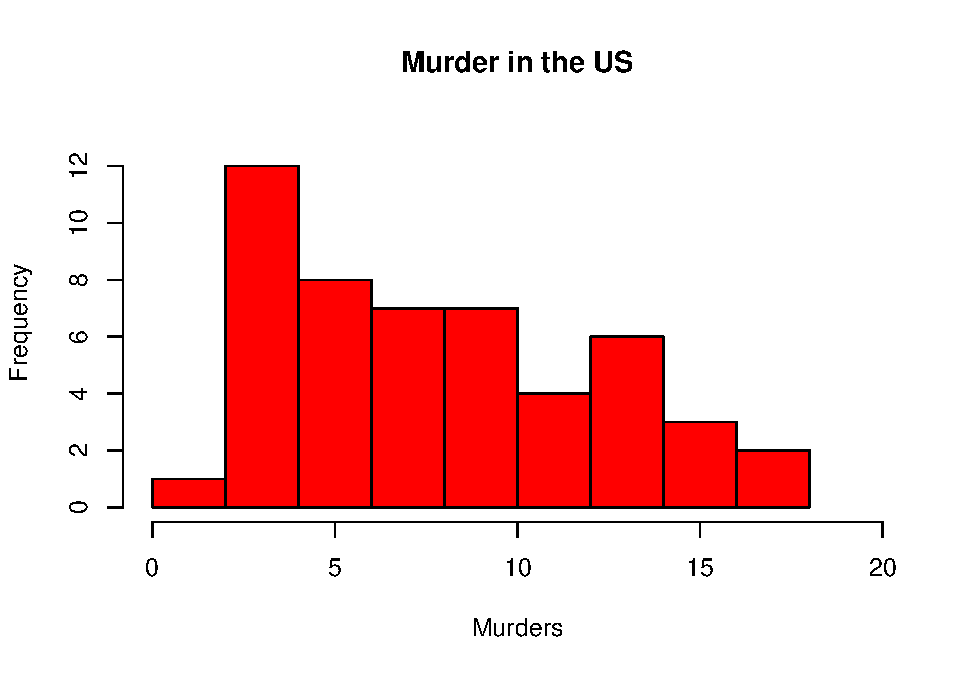
\includegraphics{Assignmentstat_files/figure-latex/unnamed-chunk-5-1.pdf}

\hypertarget{problem-6}{%
\subsubsection{Problem 6}\label{problem-6}}

Please summarize \texttt{Murder} quantitatively. What are its mean and
median? What is the difference between mean and median? What is a
quartile, and why do you think R gives you the 1st Qu. and 3rd Qu.?

\begin{Shaded}
\begin{Highlighting}[]
\FunctionTok{summary}\NormalTok{(dat.us}\SpecialCharTok{$}\NormalTok{Murder)}
\end{Highlighting}
\end{Shaded}

\begin{verbatim}
##    Min. 1st Qu.  Median    Mean 3rd Qu.    Max. 
##   0.800   4.075   7.250   7.788  11.250  17.400
\end{verbatim}

Answer: The mean for Murder is 7.788 and the median is 7.250. The mean
is the amount that each subject would have if all of the values were
added together and evenly distributed. If all 50 states had the same
frequency of arrests for murders then it would be 7.788. The median is
the middle value where exactly 50\% of the values fall either above or
below it. In the US, 50\% of states have an arrest for murder frequency
above 7.250 and the other 50\% is below that. The median is highly
robust because it is not greatly affected by outliers. The mean is the
most common measure of central tendency but it is not robust because it
will change based on the skewness of the distribution. A quartile
indicates an interval that contains 25\% or a quarter of the data.The
first quartile for ``Murder'' is 4.075 which means that 25\% of the
``Murder'' data falls below 4.075 and the 3rd quartile is 11.250 which
means that 25\% of US states have a frequency of arrests for murder that
is higher than 11.250. R gives you the 1st and 3rd quartile because
those values are useful in determining the interquartile range (IQR).
The IQR is the central half which means that 50\% of the data falls
within the 1st and 3rd quartile. In a box plot, values 1.5 IQRs above or
below the tails are considered outliers.

\hypertarget{problem-7}{%
\subsubsection{Problem 7}\label{problem-7}}

Repeat the same steps you followed for \texttt{Murder}, for the
variables \texttt{Assault} and \texttt{Rape}. Now plot all three
histograms together. You can do this by using the command
\texttt{par(mfrow=c(3,1))} and then plotting each of the three.

\begin{Shaded}
\begin{Highlighting}[]
\FunctionTok{par}\NormalTok{(}\AttributeTok{mfrow=}\FunctionTok{c}\NormalTok{(}\DecValTok{3}\NormalTok{,}\DecValTok{1}\NormalTok{))}

\FunctionTok{hist}\NormalTok{(dat.us}\SpecialCharTok{$}\NormalTok{Murder, }\AttributeTok{xlab=} \StringTok{"Murders"}\NormalTok{, }\AttributeTok{ylab=}\StringTok{"Frequency"}\NormalTok{, }\AttributeTok{main=} \StringTok{"Murder in the US"}\NormalTok{, }\AttributeTok{xlim=}\NormalTok{(}\FunctionTok{c}\NormalTok{(}\DecValTok{0}\NormalTok{, }\DecValTok{20}\NormalTok{)), }\AttributeTok{ylim=}\NormalTok{(}\FunctionTok{c}\NormalTok{(}\DecValTok{0}\NormalTok{, }\DecValTok{13}\NormalTok{)), }\AttributeTok{col=}\StringTok{"red"}\NormalTok{, }\AttributeTok{breaks=} \DecValTok{10}\NormalTok{)}

\FunctionTok{hist}\NormalTok{(dat.us}\SpecialCharTok{$}\NormalTok{Assault, }\AttributeTok{xlab=} \StringTok{"Assaults"}\NormalTok{, }\AttributeTok{ylab=}\StringTok{"Frequency"}\NormalTok{, }\AttributeTok{main=} \StringTok{"Assault in the US"}\NormalTok{, }\AttributeTok{xlim=}\NormalTok{(}\FunctionTok{c}\NormalTok{(}\DecValTok{0}\NormalTok{, }\DecValTok{350}\NormalTok{)), }\AttributeTok{ylim=}\NormalTok{(}\FunctionTok{c}\NormalTok{(}\DecValTok{0}\NormalTok{, }\DecValTok{15}\NormalTok{)), }\AttributeTok{col=}\StringTok{"blue"}\NormalTok{, }\AttributeTok{breaks=}\DecValTok{10}\NormalTok{)}

\FunctionTok{hist}\NormalTok{(dat.us}\SpecialCharTok{$}\NormalTok{Rape, }\AttributeTok{xlab=} \StringTok{"Rapes"}\NormalTok{, }\AttributeTok{ylab=}\StringTok{"Frequency"}\NormalTok{, }\AttributeTok{main=} \StringTok{"Rape in the US"}\NormalTok{, }\AttributeTok{xlim=}\NormalTok{(}\FunctionTok{c}\NormalTok{(}\DecValTok{0}\NormalTok{, }\DecValTok{50}\NormalTok{)), }\AttributeTok{ylim=}\NormalTok{(}\FunctionTok{c}\NormalTok{(}\DecValTok{0}\NormalTok{, }\DecValTok{15}\NormalTok{)), }\AttributeTok{col=}\StringTok{"green"}\NormalTok{, }\AttributeTok{breaks=}\DecValTok{10}\NormalTok{)}
\end{Highlighting}
\end{Shaded}

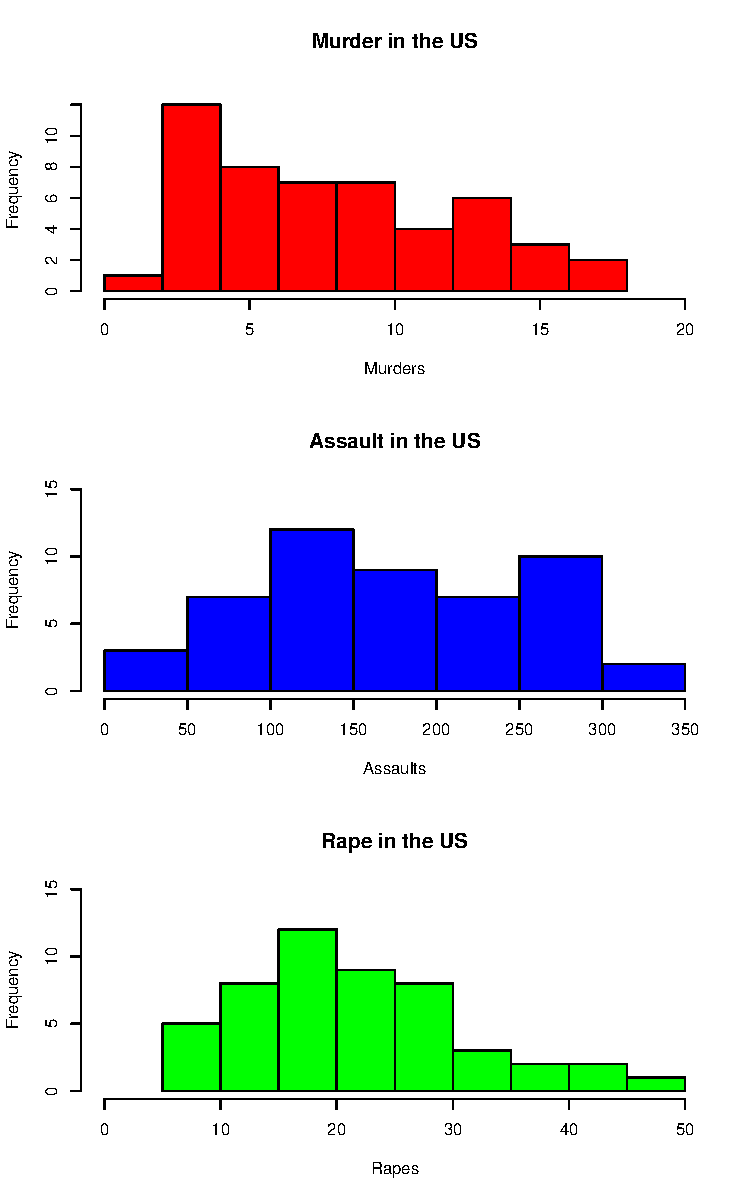
\includegraphics{Assignmentstat_files/figure-latex/unnamed-chunk-7-1.pdf}

What does the command par do, in your own words (you can look this up by
asking R \texttt{?par})?

Answer: Command par is used to set parameters. The mfrow input allows
you to create an array to plot multiple graphs on one window. The
command par(mfrow=c(3,1)) allows three graphs to be plotted in three
rows.

What can you learn from plotting the histograms together?

Answer: When the histograms are plotted together it is easier to compare
the skewness and spread of each plot. You can see where each histogram
has its peaks and outliers.

\hypertarget{problem-8}{%
\subsubsection{Problem 8}\label{problem-8}}

In the console below (not in text), type
\texttt{install.packages("maps")} and press Enter, and then type
\texttt{install.packages("ggplot2")} and press Enter. This will install
the packages so you can load the libraries.

Run this code:

\begin{Shaded}
\begin{Highlighting}[]
\FunctionTok{library}\NormalTok{(}\StringTok{\textquotesingle{}maps\textquotesingle{}}\NormalTok{) }
\FunctionTok{library}\NormalTok{(}\StringTok{\textquotesingle{}ggplot2\textquotesingle{}}\NormalTok{) }

\FunctionTok{ggplot}\NormalTok{(dat.us, }\FunctionTok{aes}\NormalTok{(}\AttributeTok{map\_id=}\NormalTok{state, }\AttributeTok{fill=}\NormalTok{Murder)) }\SpecialCharTok{+} 
  \FunctionTok{geom\_map}\NormalTok{(}\AttributeTok{map=}\FunctionTok{map\_data}\NormalTok{(}\StringTok{"state"}\NormalTok{)) }\SpecialCharTok{+} 
  \FunctionTok{expand\_limits}\NormalTok{(}\AttributeTok{x=}\FunctionTok{map\_data}\NormalTok{(}\StringTok{"state"}\NormalTok{)}\SpecialCharTok{$}\NormalTok{long, }\AttributeTok{y=}\FunctionTok{map\_data}\NormalTok{(}\StringTok{"state"}\NormalTok{)}\SpecialCharTok{$}\NormalTok{lat)}
\end{Highlighting}
\end{Shaded}

What does this code do? Explain what each line is doing.

Answer: The lines library(`maps') and library(`ggplot2') are pulling
from the packages that were installed. The line ggplot(dat.us,
aes(map\_id=state, fill=Murder)) is creating a ggplot with the USArrests
dataset. The plot is set with an aesthetic of a map with the US states.
Each state is filled in with its respective murder arrest data. The line
geom\_map(map=map\_data(``state'')) contains the map coordinates for
each US state.The last line
`expand\_limits(x=map\_data(``state'')\(long, y=map_data("state")\)lat)'
ensures that the limits of the plot include a single value for all
plots. The x and y axis of this plot contains the value of ``state''
from the map data. The x axis is longitude and the y axis is latitude.
Together this code creates a map of the US with each state filled in
with its value for murder arrests.The darker blue indicates that the
murder arrest frequency is 5 and below and the light blue indicates that
it is 15 and above.

\[\\[2in]\]

\hypertarget{assignment-2}{%
\section{Assignment 2}\label{assignment-2}}

(Coming soon)

\end{document}
